%----------------------------------------------------------------------------------------
%	PACKAGES AND OTHER DOCUMENT CONFIGURATIONS
%----------------------------------------------------------------------------------------

\documentclass{article}

\usepackage{fancyhdr} % Required for custom headers
\usepackage{lastpage} % Required to determine the last page for the footer
\usepackage{extramarks} % Required for headers and footers
\usepackage[usenames,dvipsnames]{color} % Required for custom colors
\usepackage{graphicx} % Required to insert images
\usepackage{listings} % Required for insertion of code
\usepackage{courier} % Required for the courier font
\usepackage{lipsum} % Used for inserting dummy 'Lorem ipsum' text into the template
\usepackage{hyperref} % Used to typeset URLs

% Margins
\topmargin=-0.45in
\evensidemargin=0in
\oddsidemargin=0in
\textwidth=6.5in
\textheight=9.0in
\headsep=0.25in

\linespread{1.1} % Line spacing

% Set up the header and footer
\pagestyle{fancy}
\lhead{\hmwkAuthorName} % Top left header
\chead{\hmwkClass\ (\hmwkClassInstructor\ \hmwkClassTime\): \hmwkTitle)} % Top center head
\rhead{\firstxmark} % Top right header
\lfoot{\lastxmark} % Bottom left footer
\cfoot{} % Bottom center footer
\rfoot{Page\ \thepage\ of\ \protect\pageref{LastPage}} % Bottom right footer
\renewcommand\headrulewidth{0.4pt} % Size of the header rule
\renewcommand\footrulewidth{0.4pt} % Size of the footer rule

\setlength\parindent{0pt} % Removes all indentation from paragraphs

%----------------------------------------------------------------------------------------
%	CODE INCLUSION CONFIGURATION
%----------------------------------------------------------------------------------------

\definecolor{MyDarkGreen}{rgb}{0.0,0.4,0.0} % This is the color used for comments
\lstloadlanguages{Perl} % Load Perl syntax for listings, for a list of other languages supported see: ftp://ftp.tex.ac.uk/tex-archive/macros/latex/contrib/listings/listings.pdf
\lstset{language=Perl, % Use Perl in this example
        frame=single, % Single frame around code
        basicstyle=\small\ttfamily, % Use small true type font
        keywordstyle=[1]\color{Blue}\bf, % Perl functions bold and blue
        keywordstyle=[2]\color{Purple}, % Perl function arguments purple
        keywordstyle=[3]\color{Blue}\underbar, % Custom functions underlined and blue
        identifierstyle=, % Nothing special about identifiers                                         
        commentstyle=\usefont{T1}{pcr}{m}{sl}\color{MyDarkGreen}\small, % Comments small dark green courier font
        stringstyle=\color{Purple}, % Strings are purple
        showstringspaces=false, % Don't put marks in string spaces
        tabsize=5, % 5 spaces per tab
        %
        % Put standard Perl functions not included in the default language here
        morekeywords={rand},
        %
        % Put Perl function parameters here
        morekeywords=[2]{on, off, interp},
        %
        % Put user defined functions here
        morekeywords=[3]{test},
       	%
        morecomment=[l][\color{Blue}]{...}, % Line continuation (...) like blue comment
        numbers=left, % Line numbers on left
        firstnumber=1, % Line numbers start with line 1
        numberstyle=\tiny\color{Blue}, % Line numbers are blue and small
        stepnumber=5 % Line numbers go in steps of 5
}

% Creates a new command to include a perl script, the first parameter is the filename of the script (without .pl), the second parameter is the caption
\newcommand{\perlscript}[2]{
\begin{itemize}
\item[]\lstinputlisting[caption=#2,label=#1]{#1.pl}
\end{itemize}
}

%----------------------------------------------------------------------------------------
%	DOCUMENT STRUCTURE COMMANDS
%	Skip this unless you know what you're doing
%----------------------------------------------------------------------------------------

% Header and footer for when a page split occurs within a problem environment
\newcommand{\enterProblemHeader}[1]{
\nobreak\extramarks{#1}{#1 continued on next page\ldots}\nobreak
\nobreak\extramarks{#1 (continued)}{#1 continued on next page\ldots}\nobreak
}

% Header and footer for when a page split occurs between problem environments
\newcommand{\exitProblemHeader}[1]{
\nobreak\extramarks{#1 (continued)}{#1 continued on next page\ldots}\nobreak
\nobreak\extramarks{#1}{}\nobreak
}

\setcounter{secnumdepth}{0} % Removes default section numbers
\newcounter{homeworkProblemCounter} % Creates a counter to keep track of the number of problems

\newcommand{\homeworkProblemName}{}
\newenvironment{homeworkProblem}[1][Problem \arabic{homeworkProblemCounter}]{ % Makes a new environment called homeworkProblem which takes 1 argument (custom name) but the default is "Problem #"
\stepcounter{homeworkProblemCounter} % Increase counter for number of problems
\renewcommand{\homeworkProblemName}{#1} % Assign \homeworkProblemName the name of the problem
\section{\homeworkProblemName} % Make a section in the document with the custom problem count
\enterProblemHeader{\homeworkProblemName} % Header and footer within the environment
}{
\exitProblemHeader{\homeworkProblemName} % Header and footer after the environment
}

\newcommand{\problemAnswer}[1]{ % Defines the problem answer command with the content as the only argument
\noindent\framebox[\columnwidth][c]{\begin{minipage}{0.98\columnwidth}#1\end{minipage}} % Makes the box around the problem answer and puts the content inside
}

\newcommand{\homeworkSectionName}{}
\newenvironment{homeworkSection}[1]{ % New environment for sections within homework problems, takes 1 argument - the name of the section
\renewcommand{\homeworkSectionName}{#1} % Assign \homeworkSectionName to the name of the section from the environment argument
\subsection{\homeworkSectionName} % Make a subsection with the custom name of the subsection
\enterProblemHeader{\homeworkProblemName\ [\homeworkSectionName]} % Header and footer within the environment
}{
\enterProblemHeader{\homeworkProblemName} % Header and footer after the environment
}

%----------------------------------------------------------------------------------------
%	NAME AND CLASS SECTION
%----------------------------------------------------------------------------------------

\newcommand{\hmwkTitle}{Homework\ \#1} % Assignment title
\newcommand{\hmwkDueDate}{Monday,\ February\ 5,\ 2018} % Due date
\newcommand{\hmwkClass}{COMPSCI\ 3650} % Course/class
\newcommand{\hmwkClassTime}{12:00pm} % Class/lecture time
\newcommand{\hmwkClassInstructor}{Dr. Esposito} % Teacher/lecturer
\newcommand{\hmwkAuthorName}{Kyle Coleman} % Your name
\newcommand{\hmwkDateStarted}{February 2} % Date started 
\newcommand{\hmwkTimeCompletion}{4.5 Hours} %Time till completion

%----------------------------------------------------------------------------------------
%	TITLE PAGE
%----------------------------------------------------------------------------------------

\title{
\vspace{2in}
\textmd{\textbf{\hmwkClass:\ \hmwkTitle}}\\
\normalsize\vspace{0.1in}\small{Due\ on\ \hmwkDueDate}\\
\normalsize\vspace{0.1in}\small{Started\ on\ \hmwkDateStarted}\\
\normalsize\vspace{0.1in}\small{Completion\ time:\  \hmwkTimeCompletion}\\
\vspace{0.1in}\large{\textit{\hmwkClassInstructor\ \hmwkClassTime}}
\vspace{3in}
}

\author{\textbf{\hmwkAuthorName}}
\date{} % Insert date here if you want it to appear below your name

%----------------------------------------------------------------------------------------

\begin{document}

\maketitle

%----------------------------------------------------------------------------------------
%	TABLE OF CONTENTS
%----------------------------------------------------------------------------------------

%\setcounter{tocdepth}{1} % Uncomment this line if you don't want subsections listed in the ToC

\newpage
\tableofcontents
\newpage

%----------------------------------------------------------------------------------------
%	PROBLEM 1
%----------------------------------------------------------------------------------------

% To have just one problem per page, simply put a \clearpage after each problem
\begin{homeworkProblem}
1.  (5  points)  What  is  a  network  protocol?   What  is  a  network  service?   What  is  the
difference between a service interface and implementation of a service?  Discuss these
concepts in the context of layered network architecture.
\newline

\problemAnswer{

To discuss these concepts we have to define a layered network stack. There are several different layered network architectures, but I will be referencing a common one known as the OSI (Open Systems Interconnection) model. The architecture is as follows:
\newline

7. Application Layer: Closest layer to the user. Interacts with applications and software running on the user's machine.
\newline

6. Presentation Layer: Cleans up data. This layer is responsible for translating data between networking formats.
\newline

5. Session Layer: Establishes connections for communication and is responsible for cleaning up closed connections. This is what makes socket programming possible.
\newline

4. Transport Layer: Transports data using set protocols. The most common is TCP.
\newline

3. Network Layer: Responsible for routing and distributing data over a network from one node to another.
\newline

2. Data-link Layer: Moves data between two directly connected nodes. For example, 802.3 Ethernet and 802.11 WiFi operate in the Data-link layer. For example, your home router runs in the data-link layer.
\newline

1. Physical Layer: This can be thought of as the "hardware layer". The physical layer encompasses the physical connections between machines and the electrical components that make networking possible.
\newline

A network protocol is an agreed upon set of rules for carrying out a specific task. A standardized method of communicating data prevents "disagreements" between computers and allows for more streamlined data communication. Examples of networking protocols include TCP/IP, HTTP(S), FTP/FTPS/SFTP, DNS, and many others. These protocols were developed by groups of computer scientists and heavily scrutinized by a larger community of computer scientists to ensure that they were as thorough as possible in the vetting process. Developing and getting approval/implementation of a new protocol is (usually) a very rigorous process. Network protocols run at various different layers of the network stack. 
\newline

A network service is a broad term used to describe an application that utilizes some kind of network protocol to transmit, manipulate, or analyze networked data. Some examples of a network service are E-Mail, DNS, online gaming, networked printing, VOIP, and instant messaging. These applications run at the highest level of the network stack known as the \textbf{application layer}. 
\newline

A network interface does not equal a network implementation. A network interface is similar to a class in OOP. It provides the nuts and bolts that allow an application to work with various network layers. The implementation however, is up to the application developer.

}
\end{homeworkProblem}

%----------------------------------------------------------------------------------------
%	PROBLEM 2
%----------------------------------------------------------------------------------------

\begin{homeworkProblem}
2.  (5 points) What is a network architecture?  What are the main differences between
the ISO/OSI and the TCP/IP architectures?
\newline
\problemAnswer{
A network architecture is a framework for network communication. Similar to a programming paradigm (such as Object-Oriented Programming), a network architecture encapsulates functionality of network communication and provides a standardized framework for development and use. The most common architectures are the ISO/OSI (International Organization for Standardization/Open Systems Implementation) model and the TCP/IP (Transmission Control Protocol/Internet Protocol) model, also known an the Internet Protocol Suite.
\newline

The ISO/OSI model is divided into 7 network layers:
\newline

7. Application Layer: Closest layer to the user. Interacts with applications and software running on the user's machine.
\newline

6. Presentation Layer: Cleans up data. This layer is responsible for translating data between networking formats.
\newline

5. Session Layer: Establishes connections for communication and is responsible for cleaning up closed connections. This is what makes socket programming possible.
\newline

4. Transport Layer: Transports data using set protocols. The most common is TCP.
\newline

3. Network Layer: Responsible for routing and distributing data over a network from one node to another.
\newline

2. Data-link Layer: Moves data between two directly connected nodes. For example, 802.3 Ethernet and 802.11 WiFi operate in the Data-link layer. For example, your home router runs in the data-link layer.
\newline

1. Physical Layer: This can be thought of as the "hardware layer". The physical layer encompasses the physical connections between machines and the electrical components that make networking possible.
\newline
}
\problemAnswer{
In contrast, the TCP/IP model is divided into four abstraction layers:
\newline

4. Application Layer: Similar to the ISO/OSI application layer. Unlike the ISO/OSI application layer, the TCP/IP application layer \textbf{does not} utilize a Presentation Layer to translate between different data types. This is expected of the developers who are implementing TCP/IP through the use of application protocol interfaces (APIs). The TCP/IP application layer handles similar responsibilities covered by the application layer, presentation layer, and session layer of the ISO/OSI architecture.
\newline

3. Transport Layer: The transport layer handles responsibilities similar to the transport layer in the ISO/OSI model. It is responsible for establishing end-to-end communication, normally in the form of a TCP connection or a User Datagram Protocol (UDP) connection.
\newline

2. Internet Layer: The internet layer handles communication across networks. It does this by utilizing IP addressing, packet routing, and various networking protocols. By using packet forwarding and routing, the internet layer makes it possible to communicate between IP addresses established on different networks. This is essentially the foundation of the Internet. 
\newline
\newpage

1. Link Layer:
This is the lowest layer in the TCP/IP architecture. The link layer is responsible for directing packets across local area networks. This link is responsible for arranging data packets into well defined "chunks" complete with essential information like packet headers. The link layer then sends the packet along to the internet layer where it can be distributed according to its header. 
}

\problemAnswer{
In conclusion, the TCP/IP architecture is conceptually very similar to the ISO/OSI. The main differences in the encapsulation of functionality. The ISO/OSI architecture is more rigid and well defined by utilizing 7 different layers to enforce proper network communication. The TCP/IP architecture relies more heavily on users and developers to implement certain services like data translation. 
}
\end{homeworkProblem}

%----------------------------------------------------------------------------------------
%	PROBLEM 3
%----------------------------------------------------------------------------------------
\begin{homeworkProblem}
3. (10 points) Answer Problem P23 from chapter 1 in your Kurose - Ross textbook.

\problemAnswer{
a) The inter-arrival time is determined by the equation $time = \frac{packetSize}{R_s}$

b) It is possible for the second packet to queue at the second link if there is a delay in sending the packet. If the delay is T seconds long then T must be $T >= \frac{L}{R_c} - \frac{L}{R_s}$
}
\end{homeworkProblem}


%----------------------------------------------------------------------------------------
%	PROBLEM 4
%----------------------------------------------------------------------------------------
\begin{homeworkProblem}
4.  (10  points)  Answer  Problem  P29  from  chapter  1  in  your  Kurose  -  Ross  textbook.
(Hint:  Recall that a geostationary satellite is 36,000 kilometers away from earth surface).
\newline
\problemAnswer{
The distance between a geostationary satellite and Earth is $3.6*10^7$
\newline
Propagation Speed is $2.4 * 10^8$ meters per second
\newline
Data rate is $10$ Mbps

\newline

Propagation Delay is calculated as $\frac{Distance}{Propagation Speed}$ 

So Propagation Delay is $\frac{3.6*10^7 meters}{2.4*10^8 meters/sec} = 0.15sec$
\newline

The bandwidth-delay product is $Propagation Delay * data rate = .15 * 10^7 (bits) = 1,500,000 bits$
\newline 

If a photo is sent every 60 seconds and the transmission rate is $10^7$ bits/sec then the minimum size of a photo for non-stop transmission must be $60*10^7 = 600,000,000bits$ or $75$ MB
}
\end{homeworkProblem}

%----------------------------------------------------------------------------------------
%	PROBLEM 5
%----------------------------------------------------------------------------------------
\begin{homeworkProblem}
5.  (10  points)  Suppose  that  a  certain  communications  protocol  involves  a  per-packet
overhead of 100 bytes for headers.  We send 1 million bytes of data using this protocol;
however, when one data byte is corrupted, the entire packet containing it is lost.  Give
the total number of overhead + loss bytes for packet data sizes (i.e.  the size of only
the data portion of the packet) of 1000, 5000, 10000, and 20000 bytes, assuming a)
the connection loses a single byte of data, and b) the sender does not retransmit lost
packets.  Which of these sizes is optimal?  Please show your work.

\problemAnswer{

$P =$ size of packet
$N =$ number of packets sent
Overhead $= 100 x N$
Assuming you lose 1 byte from each package i.e. if you have $200$ packages sent you will lose $200$ bytes on failure.
\newline

$1000000/1000 = 1000$ packets $ = 100,000$ bytes of overhead $ + 1000$ lost bytes $ = 101,000$ bytes
$1000000/5000 = 200$ packets $ = 20,000$ bytes of overhead $ + 5,000$ lost bytes $ = 25,000$ bytes
$1000000/10000 = 100$ packets $ = 10,000$ bytes of overhead $ + 10,000$ lost bytes $ = 20,000$ bytes
$1000000/20000 = 50$ packets $ = 5,000$ bytes of overhead $ + 20000$ lost bytes $ =  25,000$ bytes
\newline

The optimal packet size to mitigate data loss is $10,000$ bytes. 

}
\end{homeworkProblem}

%----------------------------------------------------------------------------------------
%	PROBLEM 6
%----------------------------------------------------------------------------------------
\begin{homeworkProblem}
6.  (30 points) Please read the position paper: End-to-End Arguments in System Design by J.H. Saltzer, D.P. Reed and D.D. Clark.
\url{http://cs.slu.edu/~espositof/teaching/3650/endtoend.pdf}
Write a small essay of about 250-300 words describing what is the end-to-end principle, why is it useful, and why, in your opinion, very recent work is questioning its value. See, e.g.,  DAIET,  a  system  proposed  in  this very  recent  paper  appeared  at  ACM HotNets in November 2017.
\url{ http://cs.slu.edu/~espositof/teaching/3650/p150-Sapio.pdf}

\problemAnswer{
"End-to-End Arguments in System Design" discusses the end-to-end design principle. End-to-end design suggests that "functions placed at low levels of a system may be redundant or of little value when compared with the cost of providing them at that low level." This principle is presented using a number of different scenarios. The first scenario is in regards to data integrity over a file transfer protocol. In a traditional file transfer protocol there are a number of threat vectors that may result in data loss or corruption. These include disk read errors, memory errors, and communication system errors. It is costly to implement an integrity check at each step in the file transfer process and duplicated file transfers would be uneconomical. A valid solution to this problem lies in the end-to-end design principle. Saltzer et. al, propose the use of a checksum to validate data integrity. A checksum could be produced at the source of the data and then read at the destination. The destination would then send their checksum result to the source where the source can validate data integrity by comparing the original checksum with the returned checksum. This has lower overhead and is a seemingly elegant way to handle data validation.

The paper, "In-Network Computation is a Dumb Idea Whose Time Has Come", presented by Sapio et. al, proposes heavier utilization of in-network computation as opposed to computation at the ends of communication. Sapio et. al, show that in-network computation can decrease data transfer size and results in a similar decrease in the workload of the end machines. Sapio et. al, also states that this design principle has been overlooked for decades because the hardware capability of network devices (routers, switches, etc.) have been lacking. The author suggests that this is no longer true due to the rapid increase in computational power of devices and that a lot of computational power is being underutilized by not implementing in-network computation. The main criticism of end-to-end design is that it adds more work to the end machines that could be offloaded onto the network infrastructure. 

}
\end{homeworkProblem}

%----------------------------------------------------------------------------------------
%	PROBLEM 7
%----------------------------------------------------------------------------------------
\begin{homeworkProblem}
Question 7 (15 points): Getting familiar with Wireshark (and netcat)
The purpose of this question is to have you setup Wireshark on your personal computer
(or figure out how to get access to it on a lab computer), and to give you some familiarity
with using Wireshark.  For the following questions, you will record some basic information
to show you have completed the assigned tasks using Wireshark.
\newline

(a) 5 points.
Follow the instructions at
\url{https://www.wireshark.org/download.html}
to download and setup Wireshark.  Once you have Wireshark setup, start it and select
an interface on which to record.  What is the interface on which you are recording
traffic?  Why did you choose the interface that you did?
\newline

\problemAnswer{
I chose the Wi-Fi: en0 interface because that is the interface my laptop is using on my home network.
}

(b) 5 points.
While Wireshark is recording a trace, open an Internet browser and load the webpage \url{www.nytimes.com}.  After the wepage has loaded, stop the trace recording.
i. List the different protocols that you see.
ii.In  which  layer  of  the  network  protocol  stack  does  each  protocol  belong?   Are
there  protocols  for  which  you  cannot  determine  the  appropriate  layer?   If  so,
which protocols?
\newline

\problemAnswer{
i. The protocols I see are: Address Resolution Protocol (ARP), UDP, TCP, DNS, NetBIOS Name Service (NBNS), and the Transport Layer Security (TSLv1) protocol.
\newline

ii. The ARP protocol runs in the Link-Layer. The UDP and TCP protocols run in the Transport Layer. DNS runs in the application layer. I am not positive about where the NBNS and TSL protocols run. I can guess that NBNS runs on the application layer, since it serves a similar purpose as the DNS protocol. Juding by the name of the TSL protocol, I assume that it runs in the Transport Layer. 
}
\newline

(c) 5 points.
Start Wireshark recording a trace.  Enter the display filter \texttt{tcp.port==80} and http into Wireshark.  While Wireshark is running,  open a terminal.  Type \texttt{nc www.google.com 80} at the terminal prompt.
From the nc manual page (type man nc in a Linux or MAC terminal) we know that:
The nc (or netcat) utility is used for just about anything under the sun involving TCP
or UDP. It can open TCP connections, send UDP packets, listen on arbitrary TCP
and UDP ports, do port scanning, and deal with both IPv4 and IPv6. Unlike telnet,
nc scripts nicely, and separates error messages onto standard error instead of sending
them to standard output, as telnet does with some. As the nc command  hangs,  type  the  following  HTTP  GET  request.   Make sure  to press enter twice after typing it.
\texttt{GET / HTTP/1.0}
\texttt{Host: www.google.com}
Take a screenshot of the packet you see in Wireshark that is generated by this command, and include the screenshot in your homework assignment.
\newline

\problemAnswer{
\begin{center}
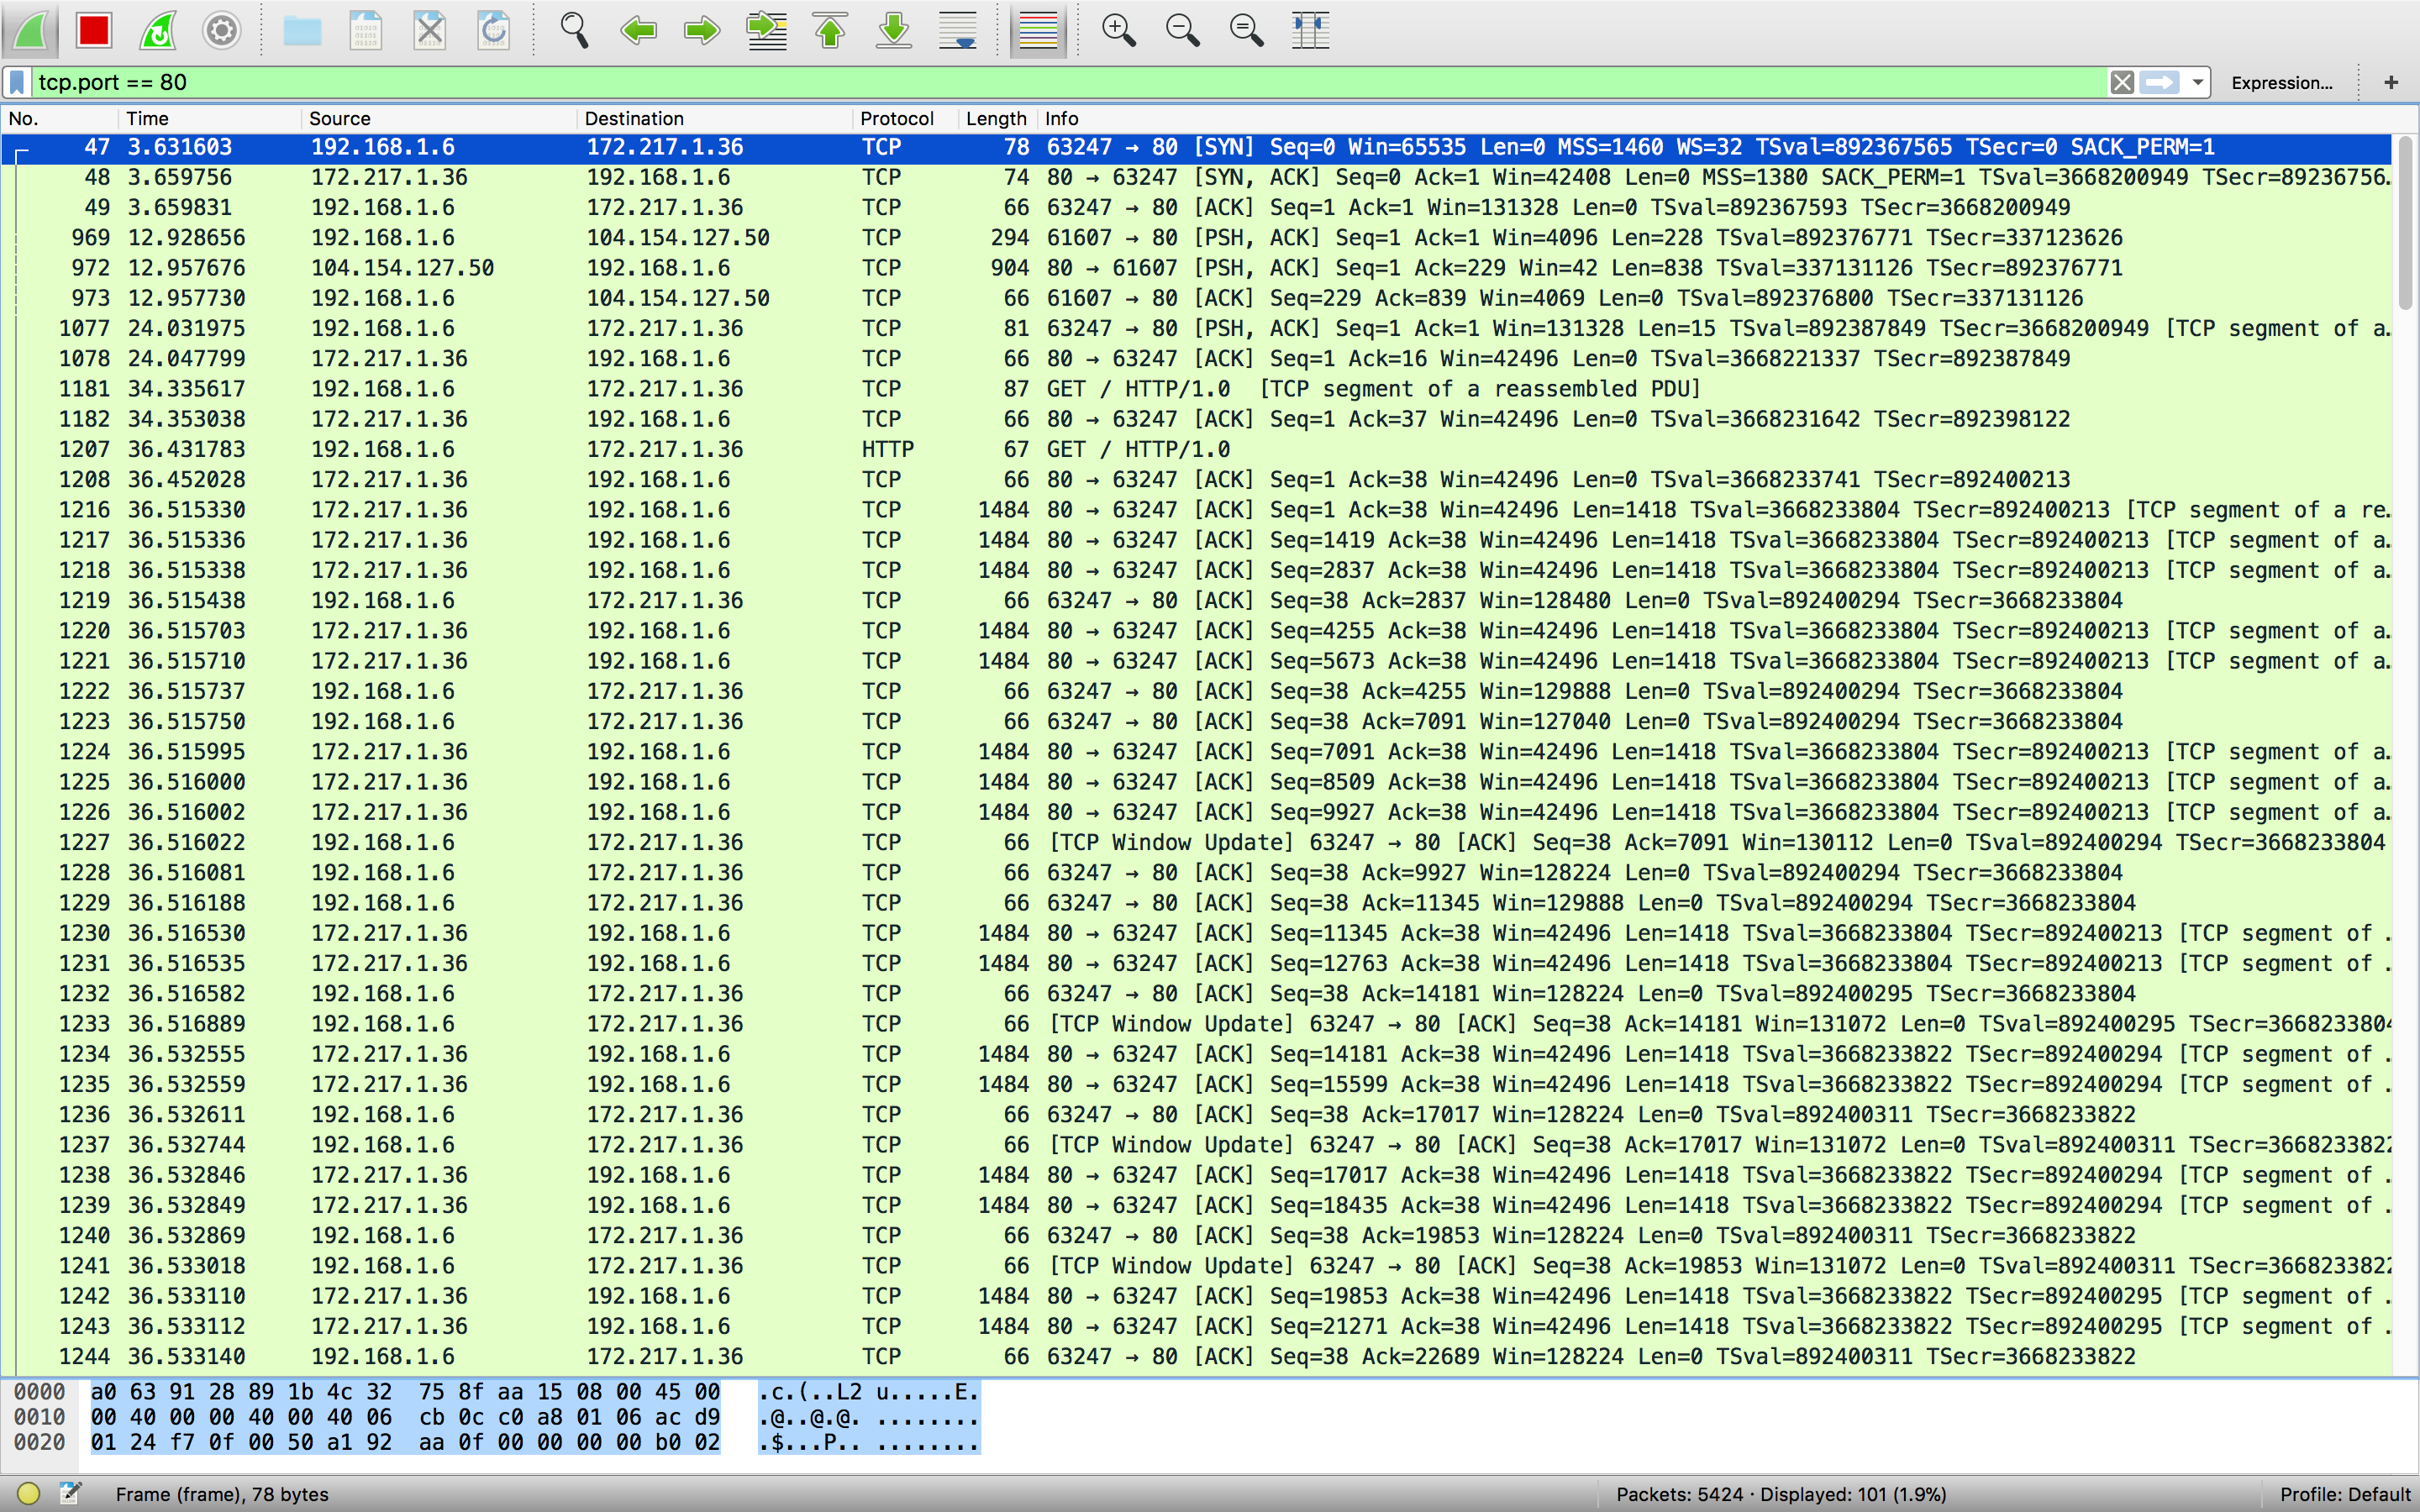
\includegraphics[scale=.25]{wireshark_screen_1}
\end{center}
}
\end{homeworkProblem}

\newpage
%----------------------------------------------------------------------------------------
%	PROBLEM 8
%----------------------------------------------------------------------------------------
\begin{homeworkProblem}
Question 8 (15 points): Playing with traceroute
\newline

The goal of this question is to use traceroute to collect some round-trip time (RTT) delays.
To find more information about traceroute,  type man traceroute at a terminal prompt.
For this question you probably should be on a network outside slu.edu since the firewall may block traceroute.
\newline

(a) 5 points.
Briefly  describe  how  traceroute  works.   What  exactly  is  being  blocked
within hopper.slu.edu that prevents traceroute to work?
\newline

\problemAnswer{
Traceroute is used to determine the number of "hops" between the destination and source of a packet. To do this, Traceroute ellicits a ICMP TIME\textunderscore EXCEEDED message. This message signifies that the packet has made the allowed number of hops and has still not found its destination. This predefined number of hops is known as the packet's time-to-live (TTL). This is necessary because if a routing packet was not told when to terminate it could potentially live on forever in search of its destination which it may never find. This is a method of cleaning up packets. Traceroute uses this feature to track the hops that a packet has to make to its destination. It does this by sending a string of packets, increasing its TTL from 1 to some arbitrary number each time the packet comes back. This allows Traceroute to know the IP of each hop along the way to the packet's destination.
\newline

The destination IP addresses are being blocked from Traceroute in SLU's network. Maybe this is because SLU's Network Department does not want the IP addresses of servers to be easily seen. This helps prevent malicious attempts against their network.
}
\newpage

(b) 5 points.
Use traceroute to connect to \url{www.stanford.edu}, at 3 different times of day.
Run traceroute 5 times at each time of day, to collect 15 sets of measurements of the round-trip time (RTT) delay to reach \url{www.stanford.edu} (ignore the other RTT measurements from the intermediate devices).  Give the 15 measurements for each time of day and calculate the average and standard deviation for each set of 15 measurements.  How many routers are in the path at each time of day?  Did the set of routers or the number of routers ever change?  Do you ever see the delay to reach a closer
host exceed the delay to reach a farther away host?  If so, what do you hypothesize that the variation is due to?
\newline

\problemAnswer{

\begin{center}
Dataset 1
\begin{tabular}{ c c c }
 M1 & M2 & M3 \\
 18.767 & 19.040 & 26.581 \\
 12.582 & 17.134 & 15.284 \\ 
 18.829 & 22.284 & 18.284 \\  
 16.259 & 20.299 & 18.684  \\
 19.959 & 20.896 & 14.202 
\end{tabular}
\end{center}
\begin{center}
Dataset2
\begin{tabular}{ccc}
 M1 & M2 & M3 \\
 14.324 & 19.394 & 13.141 \\ 
 18.392 & 22.394 & 23.193 \\
 19.193 & 16.786 & 17.413 \\
 22.983 & 22.913 & 14.254 \\
 14.129 & 20.938 & 17.496 
\end{tabular}
\end{center}
\begin{center}
Dataset 3
\begin{tabular}{ccc}
 M1 & M2 & M3 \\
 12.392 & 18.783 & 13.498 \\ 
 17.239 & 13.987 & 22.082 \\
 18.658 & 19.293 & 10.113 \\
 25.192 & 20.192 & 22. 092 \\
 22.538 & 19.103 & 20.194
\end{tabular}
\end{center}
Using R I came up with the following averages and standard deviations for each dataset:
\begin{center}
\begin{tabular}{ccc}
 Dataset & Mean & SD \\
 1 & 18.606 & 3.399 \\ 
 2 & 18.463 & 3.509\\
 3 & 18.357 & 4.209
\end{tabular}
\end{center}

\newline

There were varying numbers of routers at each time of the day. Usually, there were between 9-16 routers. 

The change in the number of routers could be due to network balancing. At busier times of the day, you may be forwarded to a different router which may change the typical path to include more hops. 

 A larger delay to reach a closer host than a farther host was not uncommon. This could also be explained by network congestion.
}
\newpage

(c) 5 points.
For one of your times of day in part (b), list out the names of intervening routers.  Based on these names, can you identify the ISPs in the path from source to destination?  There is no right or wrong answer for this question, just see what you can find out.
\newline
\problemAnswer{
\begin{center}
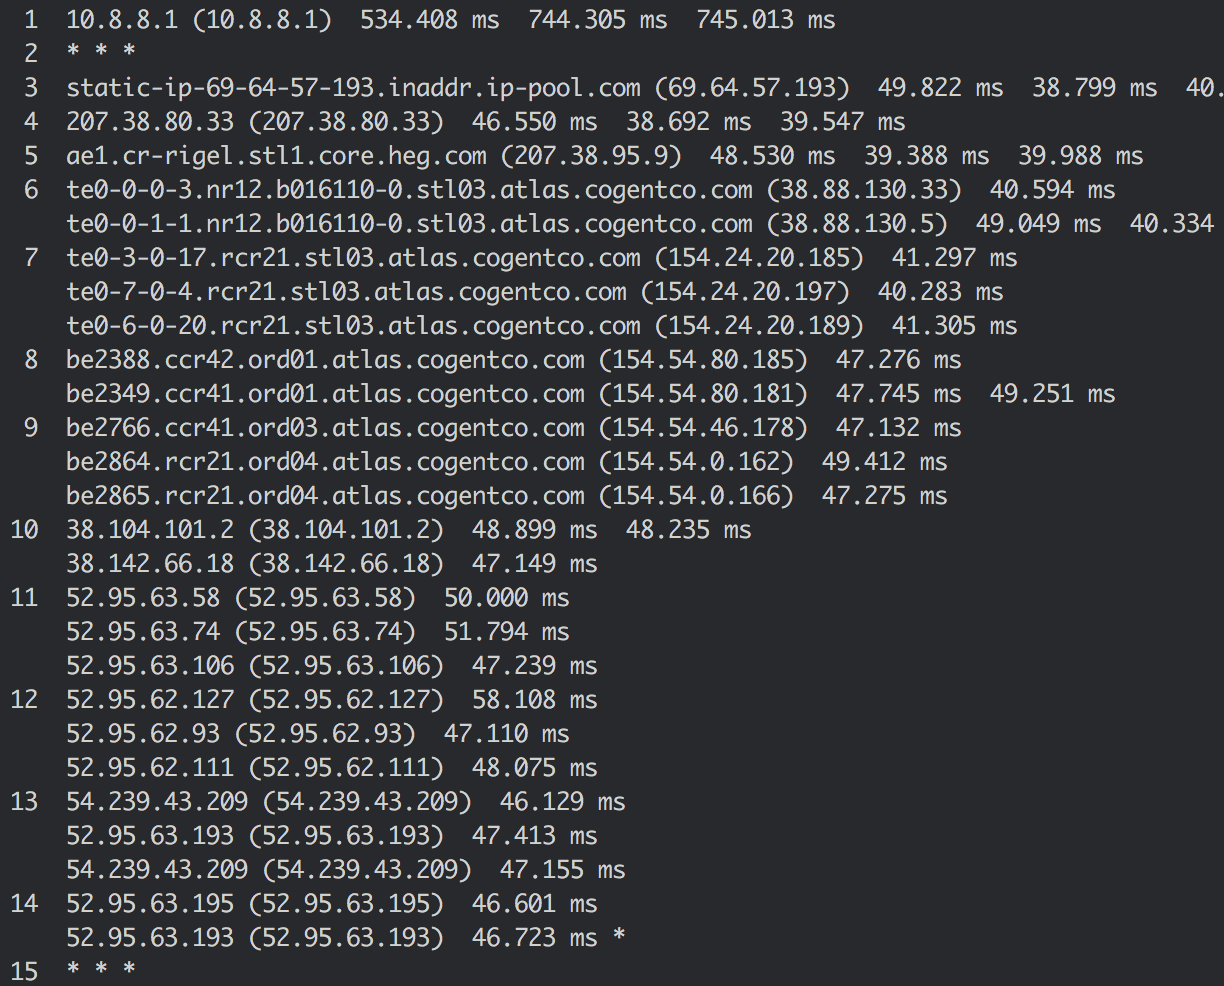
\includegraphics[scale=.3]{terminal_screen_1}
\end{center}

One of these IP's have to belong to Charter, my ISP. There is also an IP belonging to Cogent Communications, which may be the ISP for Stanford. According to an IP lookup site, some of the IPs also belonged to Amazon (likely AWS). This makes sense since they host so much of the Internet. 
}
\end{homeworkProblem}




%----------------------------------------------------------------------------------------

\end{document}